\section{Interviews}
\label{sec:interviews}

We conducted a series of semi-structured interviews on the use of Tor Browser
and onion services to \first explore user experience outside the constraints of
an online survey and to \second inform the creation of our survey---and vice
versa because we conducted some interviews after our survey ended.

\subsection{Method}

We developed a question set that served as the basis for each
interview.\footnote{The question set is available online at
\url{https://nymity.ch/onion-services/pdf/interview-checklist.pdf}.}  The
semi-structured nature of our interviews allowed us to deviate from this
question set, \eg, by asking follow-up questions.  We began by asking
demographic information (gender, age range, occupation, country of residence,
and level of education), followed by information about online behavior, and
finally questions specific to Tor Browser and onion services.

\subsubsection{Recruitment}

To select eligible interview subjects, we created a short pre-interview survey
(see Appendix~\ref{sec:interview-survey}), which was advertised by The Tor
Project both in a blog post~\cite{Winter2017a} and on its Twitter account.  Our
selection process favored laypeople and sought to maximize cultural, gender,
location, education, and age diversity.  In addition to our online screening, we
recruited participants in person at an Internet freedom event.  We found it
difficult to draw a uniform sample of Tor users to interview. We believe that
The Tor Project's blog and Twitter account are mainly followed by
disproportionately technical users while many non-technical users may install
Tor Browser in a one-off process and then cease to follow the project.  To make
matters worse, many Tor users value their privacy significantly more than the
average Internet user, making it challenging to evoke enough trust to have users
open up to us about their browsing habits.

We ended up interviewing seventeen subjects whose demographic information is
shown in Table~\ref{tab:interviewees}.  Given the sensitive nature of our
interviews, we only present aggregate information to protect the identity of our
participants.  We believe that our sample is biased towards educated and
technical users (almost 60\% of our participants have a postgraduate degree) but
it also shows the diversity among Tor's user base: Our participants comprised
human rights activists, legal professionals, writers, artists, and journalists,
just to name a few.

\begin{table*}[ht]
	\centering
	\begin{tabular}{l r r | l r r | l r r | l r r}
	\toprule
	Age & \# & \% &
	Gender & \# & \% &
	Continent of residence & \# & \% &
	Education & \# & \% \\
	\midrule
	18--25 & 2  & 11.8 & Female & 5  & 29.4 & Asia          & 3 & 17.6 & No degree    & 1  & 5.9 \\
	26--35 & 10 & 58.8 & Male   & 12 & 70.6 & Australia     & 1 &  5.9 & High school  & 3  & 17.7 \\
	36--45 & 4  & 23.5 &        &    &      & Europe        & 4 & 23.5 & Graduate     & 3  & 17.7 \\
	46--55 & 1  & 5.9  &        &    &      & North America & 8 & 47.1 & Postgraduate & 10 & 58.8 \\
	       &    &      &        &    &      & South America & 1 &  5.9 & & & \\
	\bottomrule
	\end{tabular}
	\caption{The distribution over gender, age, country of residence, and
	education for our seventeen interview subjects.  We chose not to display
	per-person demographic information to protect the identity of our interview
	subjects.}
	\label{tab:interviewees}
\end{table*}

\subsubsection{Procedure}

Princeton University's institutional review board (IRB) deemed our study exempt
from further review.\footnote{Our IRB protocol number is 8251.}  We conducted
thirteen interviews in person and four interviews remotely; over Skype, Signal,
WhatsApp, and Jitsi---depending on what our interviewees felt the most
comfortable with.  For in-person interviews we asked our interviewees to sign a
consent form.  This was not practical for remote interviews, so we sent the
consent form in advance over email and, after seeking permission from our IRB,
asked for verbal consent before the interview.  In all cases we explicitly asked
for permission to record the conversation.  All except two participants agreed
to have their interview recorded.  In the remaining two interviews we took notes
instead.  We made it clear to our participants that they could withdraw their
consent at any time.  Each interview ended with a debriefing phase in which we
asked if our participants had any remaining questions.  Some wanted to know if
technical explanations they provided earlier were correct.  Finally, we offered
our participants a gift card worth twenty dollars as a token of appreciation.

We used the services of the company Rev to have our recordings transcribed.  A
mutually-signed non-disclosure agreement protected the confidentiality of our
data.  Once our our interview recordings were transcribed, we deleted the
original recordings and employed qualitative data coding to analyze the
transcripts.  Each interview transcript was coded by two members of our team.
This process identified twenty-seven themes that are all listed in
Appendix~\ref{sec:coding-themes}.

\subsection{Results}

We now discuss how our interview participants \emph{use}, \emph{perceive}, and
\emph{(mis)understand} both Tor and onion services.

\subsubsection{Understanding}

\begin{figure}[t]
    \centering
    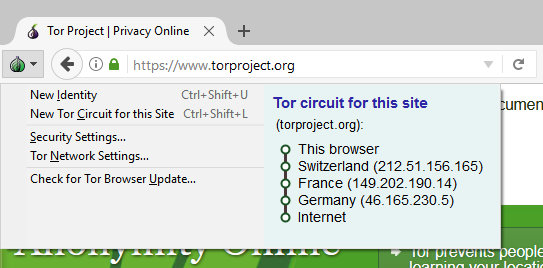
\includegraphics[width=\linewidth]{figures/tor-button-screenshot.jpg}
    \caption{A click on the onion icon reveals the Tor relays that constitute
    the circuit that was used to fetch the current page.}
    \label{fig:tor-button}
\end{figure}

Several of our participants enjoyed the visual feedback in Tor Browser (see
Figure~\ref{fig:tor-button}) that shows the circuit that is used for a given
site.  One interviewee mentioned:

\begin{displayquote}
I love how I can monitor the network through this little kind of bar that comes
up.
\end{displayquote}

Not satisfied with only seeing the current circuit, some participants wished it
were easier to learn what else is happening behind the scenes:

\begin{displayquote}
{[It]} would be nice to have some kind of application, something on that browser,
that gives you an impression of\dots what the Tor Browser's actually doing.
\end{displayquote}

Finding the right balance between what information to show and what to hide is
challenging by itself, and only exacerbated by Tor's technically diverse user
base.  While technical users may appreciate a closer look ``under the hood,''
non-technical users, who often see Tor as a tool to get a specific job
done~\cite[\S~4.3.2]{Gallagher2017a}, can easily feel bewildered and
overwhelmed.  One aspect in which more transparency could benefit Tor's entire
user base is when sites don't load:

\begin{displayquote}
\dots maybe some sort of graphical representation of is the circuit still
being built, or is the circuit built, and the site isn't responding at all to
the third relay?
\end{displayquote}

A comprehensible feature is an indicator of the anonymity that Tor Browser can
provide in a given situation:

\begin{displayquote}
In terms of the anonymity, you can't really tell\dots That's fairly opaque, so I
can't even tell how effective that's working, or whether it is\dots
\end{displayquote}

Quantifying anonymity in a real-world setting is complex, error-prone, and often
misleading.  What's more, Tor Browser does not have available all the data it
would need to quantify its user's anonymity, \eg, intermediate autonomous
systems, personal threat models, or the number of users that browse through Tor
in the same autonomous system.  For these reasons an ``anonymity meter'' is
likely a dead end, which is why The Tor Project focuses its efforts on
documentation and education.  Having been exposed to some of this documentation,
some of our participants lamented its limitations.  Asked about the difficulties
of setting up an onion service, one participant responded:

\begin{displayquote}
Tor does a good job on their web site of telling you to modify your
[configuration] file, and then getting the onion set up.  But it's just very
basic.  I have to go [to] other people's blog post to find out.
\end{displayquote}

Comprehensive documentation is only useful if it is understood.  One participant
struggled with the lack of localization.  While Tor Browser's user interface is
available in Spanish, the documentation is not:

\begin{displayquote}
Think more [about] the Spanish community\dots because in my case I'm trying to
train people to use Tor but I work in the indigenous communities and there are
some things that [are] hard for me to explain in terms of how you use Tor\dots
\end{displayquote}

\subsubsection{Misunderstandings}

We asked our participants to draw sketches of how they believe Tor and onion
services work.\footnote{All sketches are available online at
\url{https://nymity.ch/onion-services/mental-models/}.}   Everybody drew a
sketch of Tor but some didn't draw onion services because they had no mental
model for it.  Interestingly, all participants understood that bouncing network
traffic across several relays is key to Tor's anonymity, as evidenced by
Figure~\ref{fig:tor-sketch} which stems from a participant with no technical
background. Note that some details of the sketch are incorrect.  Tor uses
three-hop circuits and circuits the forward and reverse path are the same.
Analogously, most of our participants understood that network traffic does not
leave the Tor network when connecting to onion services.
Figure~\ref{fig:os-sketch} illustrates an example, again drawn by a
non-technical participant.

\begin{figure}[t]
    \centering

    \begin{subfigure}[t]{\linewidth}
        \centering
        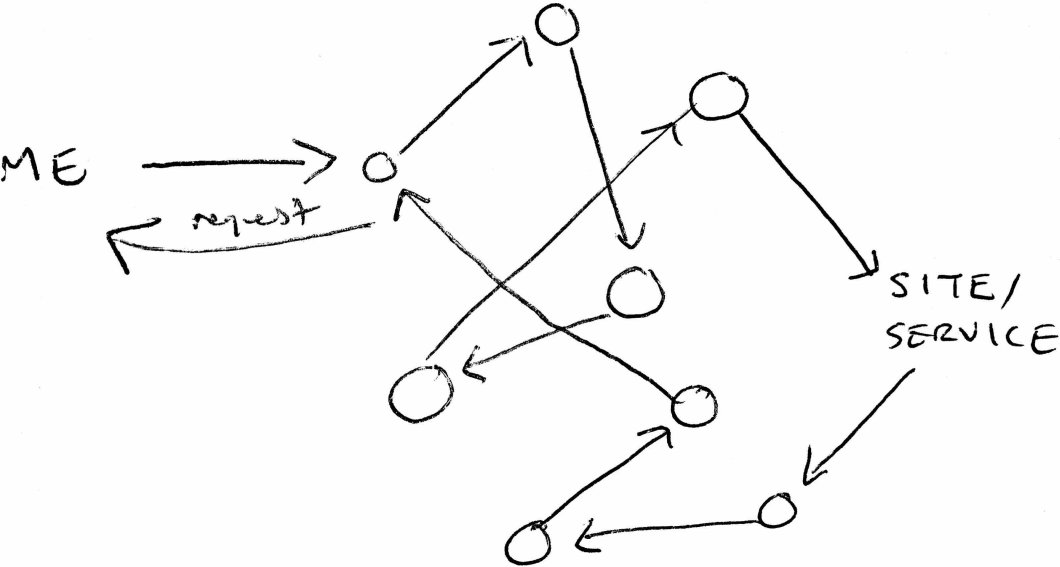
\includegraphics[width=0.8\linewidth]{figures/tor-sketch.jpg}
        \subcaption{A non-technical interview subject's sketch of how they
        believe Tor works.  The participant correctly understands the concept of
        bouncing network traffic over several hops.}
        \label{fig:tor-sketch}
    \end{subfigure}

    \begin{subfigure}[t]{\linewidth}
        \centering
        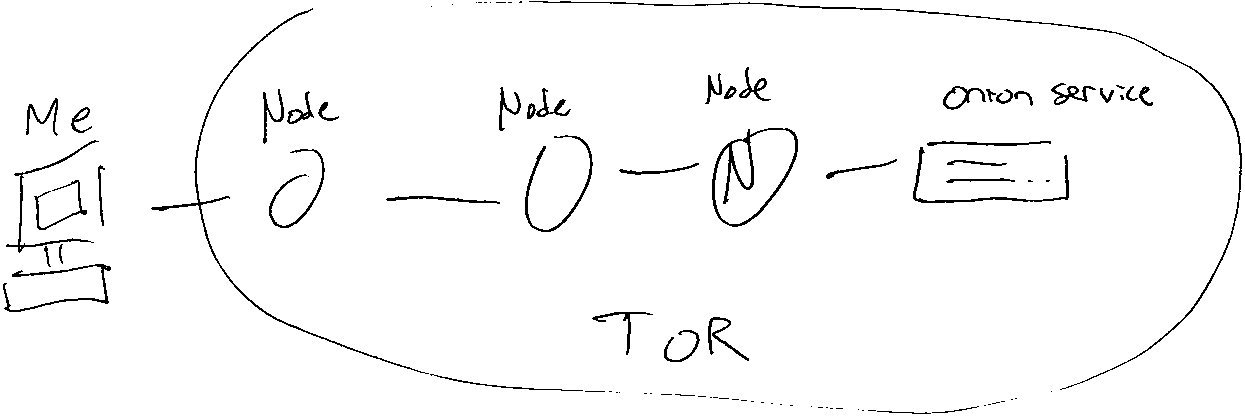
\includegraphics[width=0.8\linewidth]{figures/os-sketch.jpg}
        \subcaption{A non-technical interview subject's sketch of their mental
        model of an onion service.  Instead of a web site, the final hop is
        another Tor hop.}
        \label{fig:os-sketch}
    \end{subfigure}

    \caption{Sketches of two different, non-technical interview participants of
    how Tor works (top) and how onion services work (bottom).}
\end{figure}

Some of our interviewees did not distinguish disguising their IP address from
disguising their real-world identity, and instead used the umbrella term of
``anonymity'' to refer to both concepts.  This conflation of concepts paints an
incomplete picture of the security and privacy guarantees that Tor can provide,
as evidenced by one participant:

\begin{displayquote}
What's the point of going to Facebook using onion services when their business
model is still about collecting your data?
\end{displayquote}

There is still merit in using Facebook's onion service.  While the company
indeed learns who is logging in, they will not learn their users' location and
operating system, and users get end-to-end security outside of the often brittle
X.509 ecosystem as well as self-authenticating names.  These benefits are
difficult to convey if users don't understand the nuances in online anonymity.
Even technical users sometimes exhibit this ``all or nothing'' approach to
anonymity.

An unrelated yet hardly unexpected source of confusion is the domain format of
onion services.  Some users have come to believe that the seemingly-random
characters in onion domains is the reason why onion services are anonymous.
Accordingly, these users also believe that vanity domains are ``less anonymous''
because part of their domains is clearly not random.

\subsubsection{Perception}

Public perception of The Tor Project and the work it does is heavily tied to
adoption.  Among our interview participants, The Tor Project enjoyed a lot
of trust:

\begin{displayquote}
Because, you guys\dots have the sort of\dots not a monopoly on trust, but you
have like a really great brand name when it comes to this stuff\dots
\end{displayquote}

Upon being told what an onion service is, one participant responded:

\begin{displayquote}
So it's like the Hidden Wiki and stuff like that, where you can buy drugs
and\dots or supposedly.
\end{displayquote}

Crime taking place over Tor and particularly on onion services was a common
theme.  Most of our participants feel safer when using Tor Browser instead of
another browser.  Some further distinguished between security and privacy, with
one respondent saying that ``\emph{Mozilla and Google do a lot for security but
    not for privacy}.''  Another participant 

\subsubsection{Disadvantages}

We were particularly interested in hearing what kind of issues Tor users face.
Perhaps the most common issue is (still) browsing speed:

\begin{displayquote}
The speed of it is problematic; sometimes I have a path that allows me to watch
streaming full HD YouTube videos, and the next time five minutes later I'm
barely getting kilobytes through.
\end{displayquote}

Occasionally, Tor's reputation precedes it and prepares users for what to
expect:

\begin{displayquote}
I didn't think it was as slow as people say it was. People said it would be much
slower experience but\ldots a little bit slower, but it didn't matter for the
things that I was doing.
\end{displayquote}

In addition to the perceived slowness, several participants lamented the
old-fashioned user interface.  Tor Browser's looks were described as
``\dots\emph{it felt like it was about five years outdated},'' ``\dots\emph{it
looked like I was in 1982},'' and ``\emph{I think the colors look a bit old
fashioned and in the former Soviet Union}\dots''

Many of our participants expressed concern that their use of Tor makes them
``stick out'' or paints a target on their backs.  Asked about the disadvantages
of using Tor, one participant responded:

\begin{displayquote}
The fact that you're using Tor.  So I think that alone to [an]\dots experienced
observer might be cause in some countries to ring your doorbell and ask what
you're up to.
\end{displayquote}

Another participant expressed this concern for other privacy tools as well:

\begin{displayquote}
When you have it on your laptop, for some authorities, that is a reason to think
of you as somebody who's deserving of suspicion.  Same thing when you have
Signal, or when you use PGP, just by having [these] that means that they
sometimes are inclined to think that, ``Oh you must have something to hide
because you've used these kind of technologies.''
\end{displayquote}

Interestingly, one participant expressed that the antiquated user interface
evoked trust:

\begin{displayquote}
At the same time I thought I think that it gave them a certain amount of
credibility, like they weren't building this for the looks, but they were
building it for functionality, so what it did.  At the same time, as I thought
it was outdated in terms of how it looked, I also thought it was sort of genuine
in a way.
\end{displayquote}

In 2016, Khattak \ea documented how Tor users are often treated differently than
non-Tor users~\cite{Khattak2016a}.  One participant mentioned:

\begin{displayquote}
It is still sometimes challenging using some everyday services, because of
CAPTCHAs and those things, but I also understand that's not so much to do with
Tor, but to do with the creators of those web sites.
\end{displayquote}

\subsubsection{Advantages}

\begin{displayquote}
I feel like I'm more in control of my internet experience that way, I'm not sort
of like a will-less victim of what other people want to do with me, so I feel
I'm more empowered and have more agency when I use the Tor Browser.
\end{displayquote}
